% ---------------------------------------------------------------------------
% Experimental evaluation (design, setup, results) for the workshop paper.
% About two IEEEtran two-column pages including the figure and the table.
%
% Requires \usepackage{graphicx,booktabs,amsmath}. The figure spans both
% columns (figure*); the table fits a single column.
%
% Every number here is produced by the artifact, in this order:
%   jupyter nbconvert --execute --inplace Experiment-job-iters.ipynb  (~13 min)
%   python plot_iteration_knee.py          -> figures/iteration_knee.pdf + table
%   python fragmentation_probe.py 12 15 21 -> runs/fragmentation_summary.csv
%
% Labels: sec:eval, sec:eval-design, sec:eval-setup, sec:eval-results,
% eq:eta, fig:knee, tab:sweep. References to sec:arch-telemetry assume the
% architecture section's label.
% ---------------------------------------------------------------------------

\section{Experimental Evaluation}
\label{sec:eval}

\subsection{Design}
\label{sec:eval-design}

Variational hybrid algorithms alternate a QPU phase (circuit execution) with
a CPU phase (parameter update) for $k$ iterations. We ask how the cost of
such a job scales with $k$ when it shares a small fleet with thousands of
similar jobs, and, more specifically, how much of that cost is computation
and how much is the QPU being \emph{held}. The experiment is a one-factor
sweep: seven 3000-job batches that are identical in every attribute except
the iteration count, $k \in \{3, 6, \dots, 21\}$, each run to completion on
the same two-QPU, two-CPU fleet. Holding the job mix fixed makes $k$ the only
independent variable, so any change in per-job cost is attributable to the
iteration loop rather than to a shift in workload.

The central measurement separates two quantities that a naive accounting
conflates. For each QPU phase the device records its \emph{computation} time
$T_{\mathrm{comp}}$, the duration of circuit execution, while the broker
records the phase's \emph{occupancy} $T_{\mathrm{occ}}$: the interval from
device selection to release, during which the job holds its qubit
reservation and the device is powered on its behalf. The two differ by the
time the job spends inside the phase waiting for a connected region of free
qubits (Section~\ref{sec:arch-telemetry}). Their ratio,
\begin{equation}
\eta \;=\; \frac{\sum T_{\mathrm{comp}}}{\sum T_{\mathrm{occ}}} \in (0, 1],
\label{eq:eta}
\end{equation}
is the fraction of reserved, powered QPU time that performs computation.
Per-job energy is charged on $T_{\mathrm{comp}}$ alone.

One consequence of the design must be stated up front. The QPU timing model
depends only on job attributes, and every job executes exactly $k$ identical
QPU phases, so $\sum T_{\mathrm{comp}}$ is linear in $k$ \emph{by
construction}; it is a control, not a finding. Its value is that it fixes the
workload term exactly: any super-linear growth in occupancy or turnaround is
thereby isolated to the resource-allocation dynamics of the fleet.

\subsection{Setup}
\label{sec:eval-setup}

\paragraph{Fleet}
Two QPUs modeled on IBM Eagle~r3 processors (\texttt{IBM\_Strasbourg},
\texttt{IBM\_Brussels}): 127 qubits each on the heavy-hex coupling map
(144 edges), 220\,000 CLOPS. Two classical nodes modeled on an
8-core/16-thread AMD Ryzen (3.8--5.0\,GHz, IPC factor 1.10), each exposing
128 CPU units and 205 memory-bandwidth units.

\paragraph{Workload}
Each batch holds 3000 jobs with $n \sim U\{10,\dots,20\}$ qubits, depth
$D \sim U\{10,\dots,20\}$, and $S \sim U\{2000,\dots,9000\}$ shots. Arrivals
follow a Poisson-like process (mean inter-arrival 0.96\,s, coefficient of
variation 1.01) over a 2885\,s window, i.e.\ 1.04 jobs/s. The seven batches
share these values row for row and differ only in the iteration count.

\paragraph{Phase models}
A QPU phase takes $\tau_{\mathrm{q}} = 10\,S \log_2 D / \mathrm{CLOPS}$
seconds (mean 0.971\,s, range 0.30--1.77\,s). A CPU phase performs
$W = 2^{n} D \cdot 1.5\times10^{-6}$ units of work in $W / (4.84\,u^{0.85})$
seconds, where $u$ is the core allocation. The dispatcher does not carry the
batch file's core column into the job object, so $u$ is drawn uniformly from
$\{4,\dots,16\}$ at each phase (mean 0.156\,s). This draw is the only
stochastic element of the sweep: QPU timing and energy are bit-identical
across runs, and blocking-dependent quantities vary by about 1\%.

\paragraph{Scheduling}
The broker polls every 0.5\,s for a device with spare capacity, prefers the
most-free one, and hands the job to it. A QPU admits the job only once a
\emph{connected} subgraph of $n$ free qubits exists, retrying once per second
until it does; the region is released at the end of every QPU phase and
re-acquired at the next iteration. A CPU phase reserves 8 units and 20
memory-bandwidth units.

\paragraph{Energy and price}
Baseline power is 70\,kW (QPU-1), 60\,kW (QPU-2), 5.0\,kW (CPU-1), and
6.5\,kW (CPU-2), at \$0.18/kWh. A job is charged its device's full baseline
power for the duration of its own computation. This is a per-job
attribution---the energy the job would draw as the device's sole tenant---and
because concurrent tenants each carry the full baseline, per-job figures are
not summed into facility totals; fleet power is the monitor's quantity
(Section~\ref{sec:arch-telemetry}).

\begin{figure*}[t]
\centering
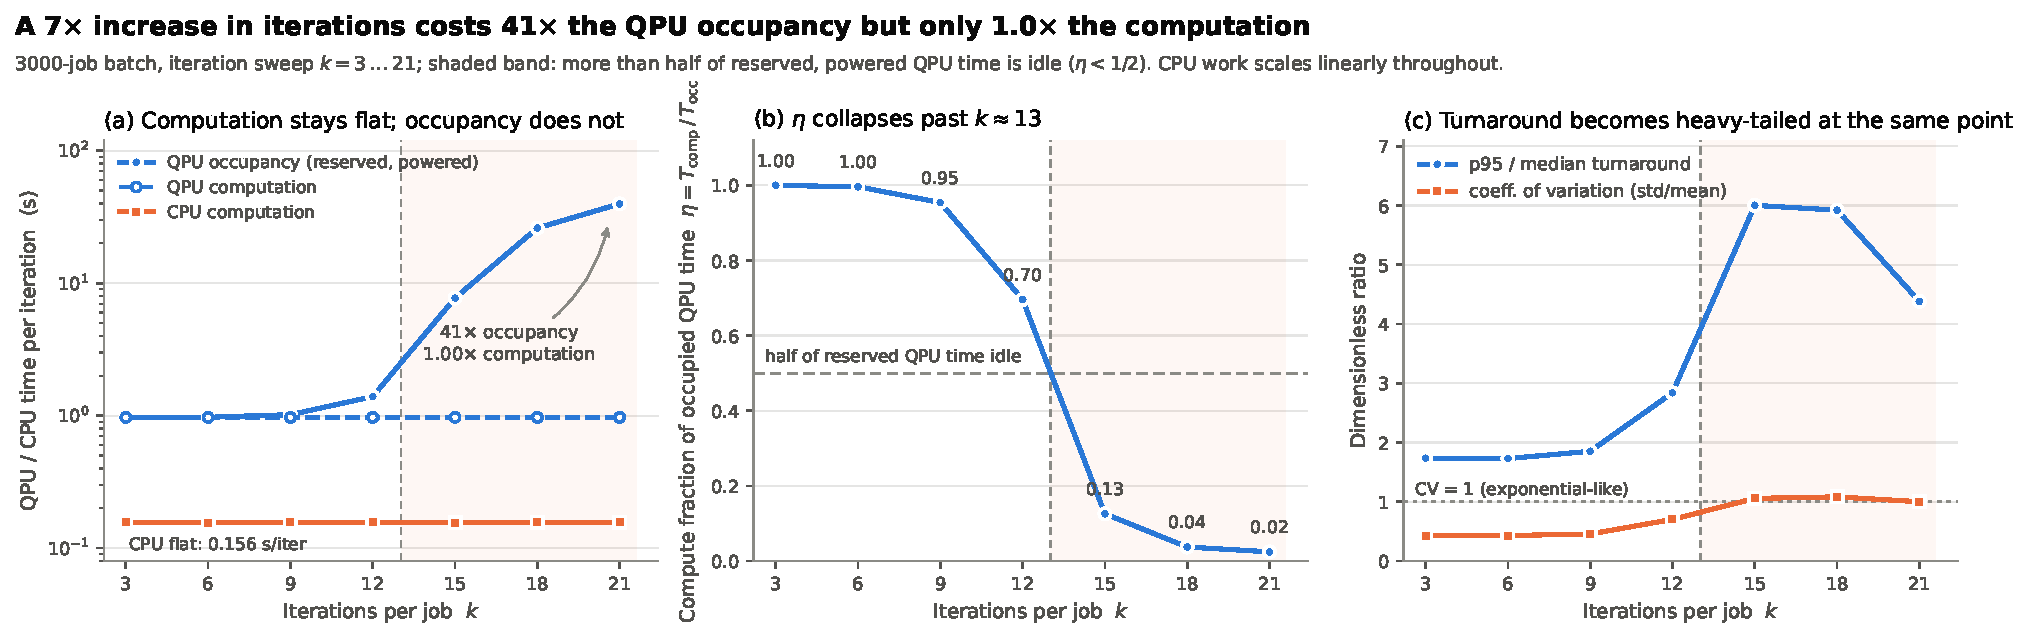
\includegraphics[width=\textwidth]{figures/iteration_knee}
\caption{Iteration sweep on the two-QPU fleet. (a)~QPU time per iteration:
computation is constant at 0.971\,s for every $k$ while occupancy---the time
a job holds its qubit reservation on a powered device---rises $41\times$; CPU
computation is flat at 0.156\,s. (b)~The compute fraction of occupied QPU
time, $\eta$ of Eq.~\eqref{eq:eta}, falls through one half near $k\approx13$
and reaches 0.024 at $k=21$. (c)~Turnaround becomes heavy-tailed in the same
bracket: the p95/median ratio and the coefficient of variation both break
upward between $k=12$ and $k=15$. The shaded band marks $\eta<\tfrac12$.}
\label{fig:knee}
\end{figure*}

\subsection{Results}
\label{sec:eval-results}

Figure~\ref{fig:knee} and Table~\ref{tab:sweep} summarize the sweep.

\paragraph{Computation is flat; occupancy is not}
QPU computation per iteration is 0.971\,s at every $k$ and CPU computation
0.156\,s: the workload term behaves exactly as the design guarantees. Per-job
attributable energy follows, growing from 0.053 to 0.373\,kWh---a factor of
6.99 for a $7\times$ increase in iterations, with $E/k$ constant to
better than 0.1\%. Occupancy tells a different story. Through $k=9$ a job holds the QPU
for 0.97--1.02\,s per iteration, essentially its computation time; at $k=12$
this reaches 1.39\,s, at $k=15$ it is 7.7\,s, and at $k=21$ it is
39.7\,s. That is a $41\times$ increase in the time a job holds a powered
QPU per iteration against a $1.00\times$ increase in the time it computes on
it.

\paragraph{The compute fraction collapses}
Eq.~\eqref{eq:eta} reduces the divergence to a single number. $\eta$ is
0.9999 at $k=3$, 0.954 at $k=9$, 0.696 at $k=12$, 0.126 at $k=15$, and
0.024 at $k=21$; it falls through one half at $k\approx13$. Past that knee
more than half, and by $k=18$ more than 96\%, of the time a job spends
holding reserved qubits on a cryogenically powered device is spent not
computing. The time to drain the batch rises accordingly, from 2888\,s at
$k=3$ to 4049\,s at $k=21$.

\paragraph{Turnaround becomes heavy-tailed at the same point}
The p95/median turnaround ratio holds at 1.7--1.9 through $k=9$, reaches 2.8
at $k=12$, and jumps to 6.0 at $k=15$; the coefficient of variation crosses
1.0 in the same bracket, the signature of an exponential-like tail. These
distributional quantities do not depend on how energy is attributed, and they
match the pre-correction runs to within the stochastic drift noted above.
The ratio narrows again at $k=21$ (4.4) not because the tail shortens but
because the bulk has joined it: from $k=18$ to $k=21$ the median turnaround
more than doubles (267 to 574\,s) while the 95th percentile grows
$1.6\times$ (1581 to 2514\,s). For scale, a $k=21$ job needs 23.7\,s of
computation and waits a median of 574\,s to obtain it; at $k=3$ the median
turnaround, 3.36\,s, is essentially the computation itself (3.38\,s).

\paragraph{Mechanism}
Because computation is fixed, the collapse must originate in re-acquisition:
a $k$-iteration job releases and re-acquires its qubit region $k$ times, and
offered QPU load grows with $k$ while capacity does not. With
$\lambda = 1.04$ jobs/s, $\tau_{\mathrm{q}} = 0.97$\,s, and roughly
$2\lfloor 127/15 \rfloor = 16$ concurrent tenants fleet-wide, utilization
$\lambda k \tau_{\mathrm{q}}/16$ reaches unity near $k=16$; topological
packing losses bring the observed knee forward to $k\approx13$. Instrumenting
the allocator shows what that loss is made of. Every blocked acquisition
attempt (each costing the job one second inside its phase) was classified by
whether the device still held enough \emph{free} qubits for the request. At
the onset of the knee, $k=12$, it did in 69.7\% of the 14\,963 blocked
attempts: on average 26.0 qubits were free against 18.1 requested, but the
largest \emph{connected} free region held only 12.4. This is connectivity
fragmentation, a failure mode with no classical analogue---a heavy-hex
lattice that is 20\% free can be unable to seat an 18-qubit circuit. As load
deepens the balance shifts to plain capacity exhaustion: fragmentation
accounts for 34.8\% of 296\,833 blocked attempts at $k=15$ and 14.9\% of
2.28~million at $k=21$. Fragmentation initiates the collapse; saturation
sustains it.

\paragraph{Implication}
Increasing the iteration count of a hybrid job does not make it more
expensive to compute; past the knee it makes it far more expensive to
\emph{hold}, and it is the holding---reserved qubits on a powered cryostat
performing no work---that dominates both the device-side cost and the tail
of turnaround. An accounting that charges the phase window rather than the
computation reports this occupancy as energy and misreads an allocation
pathology as a property of the workload.

\begin{table}[t]
\caption{Iteration sweep, 3000 jobs per batch, means over jobs.
$T_{\mathrm{comp}}$ and $T_{\mathrm{occ}}$ are QPU seconds per iteration;
$E$ is per-job attributable energy; p95/med and CV describe job turnaround.}
\label{tab:sweep}
\centering
\begin{tabular}{@{}rrrrrrr@{}}
\toprule
$k$ & $T_{\mathrm{comp}}$ & $T_{\mathrm{occ}}$ & $\eta$ & $E$ (kWh) & p95/med & CV \\
\midrule
 3 & 0.971 &  0.971 & 1.000 & 0.053 & 1.73 & 0.43 \\
 6 & 0.971 &  0.974 & 0.996 & 0.107 & 1.73 & 0.43 \\
 9 & 0.971 &  1.017 & 0.954 & 0.160 & 1.85 & 0.46 \\
12 & 0.971 &  1.394 & 0.696 & 0.213 & 2.84 & 0.70 \\
15 & 0.971 &  7.727 & 0.126 & 0.267 & 6.00 & 1.06 \\
18 & 0.971 & 26.09  & 0.037 & 0.320 & 5.92 & 1.08 \\
21 & 0.971 & 39.73  & 0.024 & 0.373 & 4.38 & 1.00 \\
\bottomrule
\end{tabular}
\end{table}
